\section{Cache模拟与测试}
\begin{center}
    每个用例的每一指标5分(最后一个用例10分)\\
    与参考csim-ref模拟器输出指标相同则判为正确
\end{center}

\subsection{Cache模拟器设计}

% 提交csim.c

\subsubsection{程序设计思想}

按照cache的层次结构,首先设计cache的数据结构,CacheLine,CacheSet,Cache,而后根据LRU算法,对cache的存取进行模拟,先判断是否命中,若命中则hit加一,否则看cache是否已经存满,不满则直接将要读的内存地址存入,否则根据LRU替换数据。

\subsubsection{输出截图}

\begin{figure}[H]
    \centering
    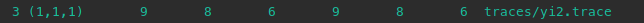
\includegraphics[width=0.7\linewidth]{figures/CSim_1}
    \caption{测试用例1的输出截图(5分)}
    \label{fig:csim1}
\end{figure}

\begin{figure}[H]
    \centering
    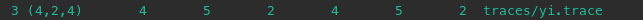
\includegraphics[width=0.7\linewidth]{figures/CSim_2}
    \caption{测试用例2的输出截图(5分)}
    \label{fig:csim2}
\end{figure}

\begin{figure}[H]
    \centering
    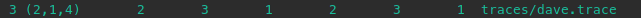
\includegraphics[width=0.7\linewidth]{figures/CSim_3}
    \caption{测试用例3的输出截图(5分)}
    \label{fig:csim3}
\end{figure}

\begin{figure}[H]
    \centering
    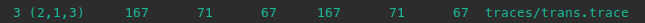
\includegraphics[width=0.7\linewidth]{figures/CSim_4}
    \caption{测试用例4的输出截图(5分)}
    \label{fig:csim4}
\end{figure}

\begin{figure}[H]
    \centering
    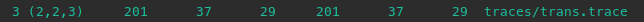
\includegraphics[width=0.7\linewidth]{figures/CSim_5}
    \caption{测试用例5的输出截图(5分)}
    \label{fig:csim5}
\end{figure}

\begin{figure}[H]
    \centering
    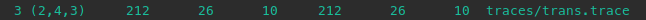
\includegraphics[width=0.7\linewidth]{figures/CSim_6}
    \caption{测试用例6的输出截图(5分)}
    \label{fig:csim6}
\end{figure}

\begin{figure}[H]
    \centering
    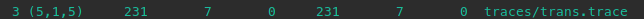
\includegraphics[width=0.7\linewidth]{figures/CSim_7}
    \caption{测试用例7的输出截图(5分)}
    \label{fig:csim7}
\end{figure}

\begin{figure}[H]
    \centering
    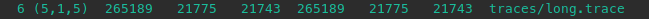
\includegraphics[width=0.7\linewidth]{figures/CSim_8}
    \caption{测试用例8的输出截图(10分)}
    \label{fig:csim8}
\end{figure}

\subsection{矩阵转置设计}

% 提交trans.c

\subsubsection{程序设计思想}

根据缓存参数可以确定缓存包含32个组,每组一行(E=1),缓存块大小为32字节,即一个缓存块能存放8个int变量。

\paragraph{32x32}首先可以推出矩阵在Cache中的存储情况如左表所示,这里可以将该矩阵分成8x8的16个小矩阵,这样每次读8个值就能充分利用缓存块,同时写的时候也可以充分利用缓存减少miss次数。

\begin{figure}[H]
    \begin{minipage}[c]{0.4\linewidth}
        \begin{tabular}{|c|c|c|c|c|}
            \hline 
            & 0-7 & 8-15 & 16-23 & 24-32 \\ 
            \hline 
            0 & 1 & 2 & 3 & 4 \\ 
            \hline 
            1 & 5 & 6 & 7 & 8 \\ 
            \hline 
            2 & 9 & 10 & 11 & 12 \\ 
            \hline 
            3 & 13 & 14 & 15 & 16 \\ 
            \hline 
            4 & 17 & 18 & 19 & 20 \\ 
            \hline 
            5 & 21 & 22 & 23 & 24 \\ 
            \hline 
            6 & 25 & 16 & 17 & 18 \\ 
            \hline 
            7 & 29 & 30 & 31 & 32 \\ 
            \hline 
            8 & 1 & 2 & 3 & 4 \\ 
            \hline 
        \end{tabular} 
    \end{minipage}
\end{figure}

\paragraph{64x64}首先可以推出矩阵在Cache中的存储情况如下表所示,这里可以将该矩阵分成8x8的64个小矩阵,然而这样会使得读取矩阵的下面4行产生miss,如果采用4x4矩阵则会导致无法充分利用缓存,即一个缓存行可以存放8个int值,而我们没有充分利用到,所以可以整体性的分成8x8,在进行转置的时候可以考虑使用矩阵的一半来做,即4x8的小块来做。

\begin{figure}[H]
\begin{tabular}{|c|c|c|c|c|c|c|c|c|}
\hline 
& 0-7 & 8-15 & 16-23 & 24-32 & 33-40 & 41-48 & 49-56 & 57-63\\ 
\hline 
0 & 1 & 2 & 3 & 4 & 5 & 6 & 7 & 8\\
\hline 
1 & 9 & 10 & 11 & 12 & 13 & 14 & 15 & 16 \\ 
\hline 
2 & 17 & 18 & 19 & 20 & 21 & 22 & 23 & 24 \\ 
\hline 
3 & 25 & 26 & 27 & 28 & 29 & 30 & 31 & 32 \\ 
\hline 
4 & 1 & 2 & 3 & 4 & 5 & 6 & 7 & 8\\
\hline 
\end{tabular} 
\end{figure}

具体操作方式如下:

\begin{enumerate}
    \item 对于前4行,按行读取8个元素存入变量中,前4个元素正常转置,后面4个原地转置后存入B矩阵中。
    \item 对于后4行,对于A中后4行的左半部分,按列读取4个元素m1,m2,m3,m4从B的右上角按行读取4个元素m5,m6,m7,m8,然后将m1,m2,m3,m4写入B右上角的行,将m5,m6,m7,m8写入B左下角的行。
\end{enumerate}

这时A矩阵的右下部分和B矩阵中的右下部分已经完全载入缓存(列不同,不会发生冲突),这个时候我们处理右下角的块时缓存命中率为100%

\paragraph{61x67}
这个矩阵是不规则的,直接用不同的分块大小测试,选用8x8的大小。

\subsubsection{输出截图}

\begin{figure}[H]
    \centering
    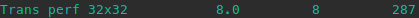
\includegraphics[width=0.7\linewidth]{figures/Trans_1}
    \caption{32×32(10分):运行结果截图}
    \label{fig:trans1}
\end{figure}

\begin{figure}[H]
    \centering
    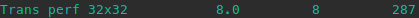
\includegraphics[width=0.7\linewidth]{figures/Trans_1}
    \caption{64×64(10分):运行结果截图}
    \label{fig:trans2}
\end{figure}

\begin{figure}[H]
    \centering
    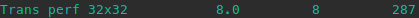
\includegraphics[width=0.7\linewidth]{figures/Trans_1}
    \caption{61×67(20分):运行结果截图}
    \label{fig:trans3}
\end{figure}
